\let\lesson\undefined
\newcommand{\lesson}{\phantomlesson{Bài 5: Chuyển động tổng hợp}}
\chapter[Chuyển động tổng hợp]{Chuyển động tổng hợp}
\setcounter{section}{0}
\section{Lý thuyết}
\subsection{Tính tương đối của chuyển động}
Một vật có thể xem như là đứng yên trong hệ quy chiếu này, nhưng lại chuyển động trong hệ quy chiếu khác. Do đó, chuyển động có tính tương đối.
\subsubsection{Quỹ đạo có tính tương đối}
Hình dạng của quỹ đạo của chuyển động trong các hệ quy chiếu khác nhau thì khác nhau. 
\subsubsection{Vận tốc có tính tương đối}
Vận tốc của chuyển động với các hệ quy chiếu khác nhau thì khác nhau. 
\subsection{Hệ quy chiếu đứng yên và hệ quy chiếu chuyển động}
\begin{itemize}
	\item \textbf{Hệ quy chiếu đứng yên:} là hệ quy chiếu gắn với vật làm mốc được quy ước là đứng yên.\\
	\textit{\textbf{Ví dụ:}} Hệ quy chiếu gắn với sân ga, hệ quy chiếu gắn với bờ sông, \dots
	\item \textbf{Hệ quy chiếu chuyển động:} là hệ quy chiếu gắn với vật làm gốc chuyển động so với hệ quy chiếu đứng yên.\\
	\textit{\textbf{Ví dụ:}} hệ quy chiếu gắn với tàu hoà đang chuyển động, hệ quy chiếu gắn với dòng nước đang trôi, \dots
\end{itemize}
\subsection{Độ dịch chuyển tổng hợp - Vận tốc tổng hợp}
Quy ước:
\begin{itemize}
	\item Vật số 1 (người) là vật chuyển động đang được xét.
	\item Vật số 2 (toa tàu) là vật chuyển động được chọn làm gốc của hệ quy chiếu chuyển động.
	\item Vật số 3 (đường ray) là vật đứng yên được chọn làm gốc của hệ quy chiếu đứng yên
\end{itemize}
\begin{center}
	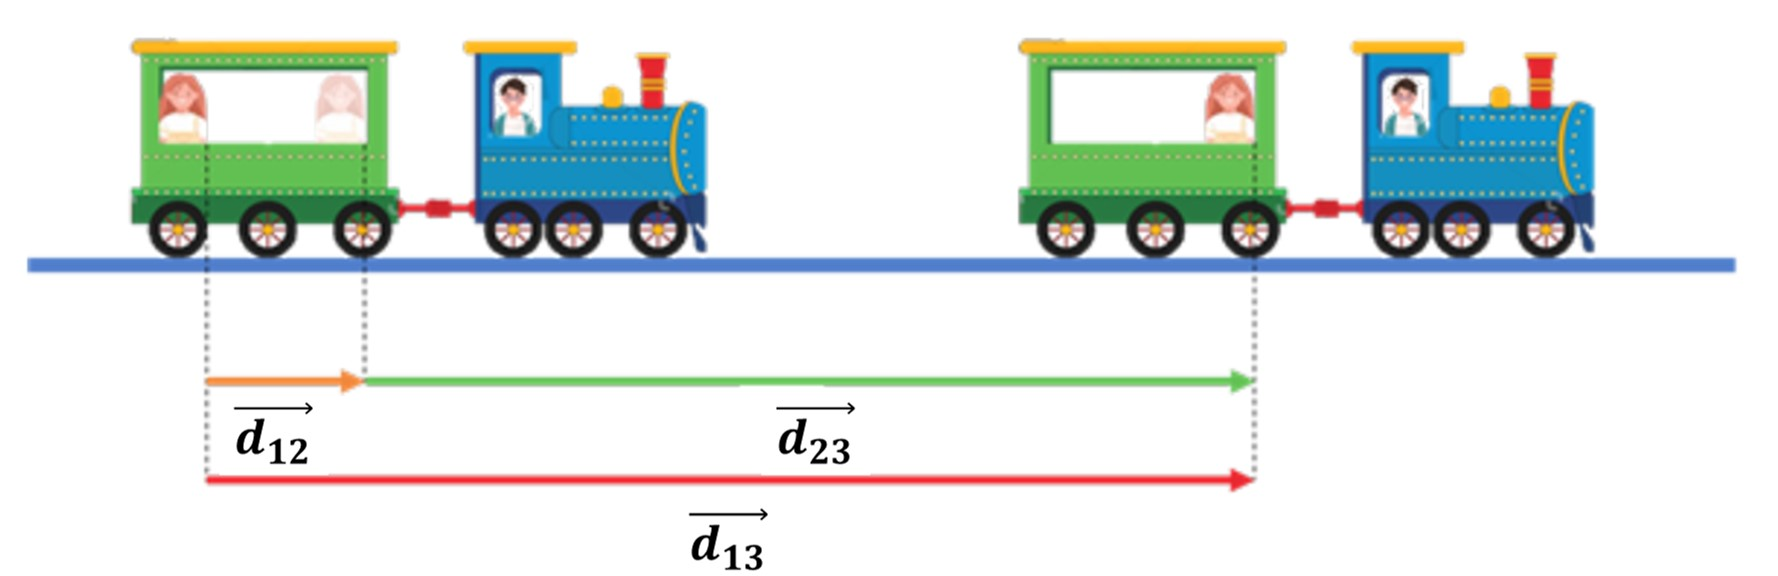
\includegraphics[width=0.6\linewidth]{../figs/VN10-2023-PH-TP006-1}
\end{center}
Khi vật 1 có độ dịch chuyển $\overrightarrow{d_{12}}$ trong hệ quy chiếu chuyển động, đồng thời hệ quy chiếu chuyển động cũng có độ dịch chuyển $\overrightarrow{d_{23}}$ so với hệ quy chiếu đứng yên. Do đó, độ dịch chuyển tổng hợp:
$$\overrightarrow{d_{13}}=\overrightarrow{d_{12}}+\overrightarrow{d_{23}}$$
Xét trong khoảng thời gian $\Delta t$ rất bé và kết hợp với định nghĩa của vận tốc:
$$\dfrac{\overrightarrow{d_{13}}}{\Delta t}=\dfrac{\overrightarrow{d_{12}}}{\Delta t}+\dfrac{\overrightarrow{d_{23}}}{\Delta t}$$
$$\Rightarrow \overrightarrow{v_{13}}=\overrightarrow{v_{12}}+\overrightarrow{v_{23}}$$
Trong đó:
\begin{itemize}
	\item $\overrightarrow{v_{13}}$: vận tốc tuyệt đối (vận tốc của vật đối với hệ quy chiếu đứng yên);
	\item $\overrightarrow{v_{12}}$: vận tốc tương đối (vận tốc của vật đối với hệ quy chiếu chuyển động);
	\item $\overrightarrow{v_{23}}$: vận tốc kéo theo (vận tốc của hệ quy chiếu chuyển động đối với hệ quy chiếu đứng yên).
\end{itemize}
\textbf{Trường hợp 1:} $\overrightarrow{v_{12}}\upuparrows \overrightarrow{v_{23}}$
	\begin{center}
		\begin{tikzpicture}
			\coordinate (O) at (0,0);
			\coordinate (B) at (2,0);
			\coordinate (C) at (5,0);
			\coordinate (D) at (2.5,0);
			\coordinate (O1) at ($(O)-(0,1cm)$);
			\coordinate (C1) at ($(C)-(0,1cm)$);
			\coordinate (D1) at ($(D)-(0,1cm)$);
			\draw[-stealth,thick, red] (O) -- (B);
			\draw[-stealth,thick, blue] (B) -- (C);
			\draw[-stealth,thick] (O1) -- (C1);
			\foreach \i in {O,O1}{
				\filldraw[black] (\i) circle (0.5mm);
			}
			\node[label={[red]90:$\overrightarrow{v_{12}}$}] at (B){};	
			\node[label={[blue]90:$\overrightarrow{v_{23}}$}] at (C){};	
			\node[label=90:$\overrightarrow{v_{13}}$] at (D1){};	
		\end{tikzpicture}
	\end{center}
$$v_{13}=v_{12}+v_{23}$$
\textbf{Trường hợp 2:} $\overrightarrow{v_{12}}\uparrow\downarrow \overrightarrow{v_{23}}$
\begin{center}
	\begin{tikzpicture}
		\coordinate (O) at (0,0);
		\coordinate (B) at (4,0);
		\coordinate (C) at (-2,0);
		\coordinate (D) at (2,0);
		\coordinate (E) at (1,0);
		\coordinate (O1) at ($(O)-(0,1cm)$);
		\coordinate (D1) at ($(D)-(0,1cm)$);
		\coordinate (E1) at ($(E)-(0,1cm)$);
		\draw[-stealth,thick, red] (O) -- (B);
		\draw[-stealth,thick, blue] (O) -- (C);
		\draw[-stealth,thick] (O1) -- (D1);
		\foreach \i in {O,O1}{
			\filldraw[black] (\i) circle (0.5mm);
		}
		\node[label={[red]90:$\overrightarrow{v_{12}}$}] at (B){};	
		\node[label={[blue]90:$\overrightarrow{v_{23}}$}] at (C){};	
		\node[label=90:$\overrightarrow{v_{13}}$] at (E1){};	
	\end{tikzpicture}
\end{center}
$$v_{13}=v_{12}-v_{23}$$
\textbf{Trường hợp 3:} $\overrightarrow{v_{12}} \bot \overrightarrow{v_{23}}$
\begin{center}
	\begin{tikzpicture}
		\coordinate (O) at (0,0);
		\coordinate (B) at (4,0);
		\coordinate (C) at (0,3);
		\coordinate (D) at (4,3);
		\coordinate (E) at (1,0);
		\coordinate (O1) at ($(O)-(0,1cm)$);
		\coordinate (D1) at ($(D)-(0,1cm)$);
		\coordinate (E1) at ($(E)-(0,1cm)$);
		\draw[-stealth,thick, red] (O) -- (B);
		\draw[-stealth,thick, blue] (O) -- (C);
		\draw[-stealth,thick] (O) -- (D);
		\draw[dashed] (B) -- (D);
		\draw[dashed] (C) -- (D);
		\foreach \i in {O}{
			\filldraw[black] (\i) circle (0.5mm);
		}
		\tkzMarkRightAngle[draw=black,size=.4](B,O,C);
		\node[label={[red,below right]90:$\overrightarrow{v_{12}}$}] at (B){};	
		\node[label={[blue]90:$\overrightarrow{v_{23}}$}] at (C){};	
		\node[label=90:$\overrightarrow{v_{13}}$] at (D){};	
	\end{tikzpicture}
\end{center}
$$v_{13}=\sqrt{v^2_{12}+v^2_{23}}$$
\textbf{Trường hợp 4:} $\left(\overrightarrow{v_{12}},\overrightarrow{v_{23}}\right)=\alpha$
\begin{center}
	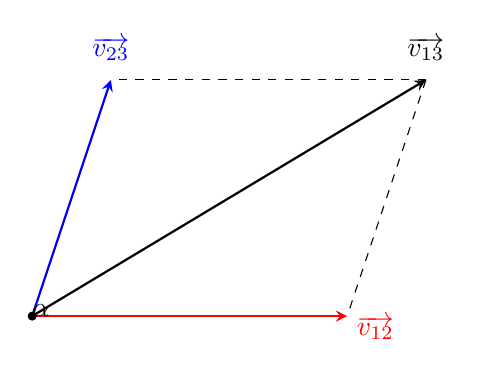
\begin{tikzpicture}
		\coordinate (O) at (0,0);
		\coordinate (B) at (4,0);
		\coordinate (C) at (5,3);
		\coordinate (D) at (1,3);
		\draw[-stealth,thick, red] (O) -- (B);
		\draw[-stealth,thick, blue] (O) -- (D);
		\draw[-stealth,thick] (O) -- (C);
		\draw[dashed] (C) -- (D);
		\draw[dashed] (C) -- (B);
		\foreach \i in {O}{
			\filldraw[black] (\i) circle (0.5mm);
		}
		\node[label={[red,below right]90:$\overrightarrow{v_{12}}$}] at (B){};	
		\node[label={[blue]90:$\overrightarrow{v_{23}}$}] at (D){};	
		\node[label=90:$\overrightarrow{v_{13}}$] at (C){};	
		\tkzMarkAngle[size=0.75cm,color=cyan](B,O,D);
		\tkzLabelAngle[color=black,pos=1.2](B,O,D){$\alpha$}
	\end{tikzpicture}
$$v_{13}=\sqrt{v^2_{12}+v^2_{23}+2v_{12}\cdot v_{23\cdot}\cos\alpha}$$
Nếu $v_{12}=v_{23}$ thì $v_{13}=2v_{12}\cdot\cos\dfrac{\alpha}{2}$.
\end{center}
\section{Mục tiêu bài học - Ví dụ minh họa}

\begin{dang}{Phân biệt vật chuyển động và đứng yên\\ trong các hệ quy chiếu khác nhau}
	\viduii{3}{Một hành khách ngồi trên toa tàu A, nhìn qua cửa sổ thấy toa tàu B bên cạnh và gạch lát sân ga đều chuyển động như nhau. Nếu lấy vật mốc là nhà ga thì:
		\begin{mcq}(2)
			\item Cả hai tàu đều đứng yên.
			\item Tàu B đứng yên, tàu A chuyển động.
			\item Tàu A đứng yên, tàu B chạy.
			\item Cả hai tàu đều chạy.
		\end{mcq}
		
	}
	{	\begin{center}
			\textbf{Hướng dẫn giải}
		\end{center}
		
		Khi hành khách ngồi trên toa tàu A, mà thấy toa tàu B bên cạnh và gạch lát sân ga đều chuyển động như nhau thì tàu B và sân ga cùng trạng thái chuyển động so với tàu A.
		
		Nếu lấy vật mốc là nhà ga, gạch lát sân ga đứng yên nên tàu B cũng đứng yên. Sân ga chuyển động so với tàu A đồng nghĩa với tàu A chuyển động so với sân ga. 
		
		Vậy trong hệ qui chiếu  gắn với sân ga (lấy vật mốc là nhà ga), tàu A chuyển động, tàu B đứng yên.
		
		
		
		\textbf{Đáp án: B}.
	}
	\viduii{2}{Hành khách 1 đứng trên toa tàu a, nhìn qua cửa số toa sang hành khách 2 ở toa bên cạnh b. Hai toa tàu đang đỗ trên hai đường tàu song song với nhau trong sân ga. Bỗng 1 thấy 2 chuyển động về phía sau. Tình huống nào sau đây chắc chắn không xảy ra?
		\begin{mcq}
			\item Cả hai toa tàu cùng chạy về phía trước. Toa a chạy nhanh hơn toa b.
			\item Cả hai toa tàu cùng chạy về phía trước. Toa b chạy nhanh hơn toa a.
			\item Toa tàu a chạy về phía trước. Toa b đứng yên.
			\item Toa tàu a đứng yên. Toa tàu b chạy về phía sau.
		\end{mcq}
	}
	{	\begin{center}
			\textbf{Hướng dẫn giải}
		\end{center}
		
		Nếu cả hai tàu cùng chạy về phía trước, tàu b chạy nhanh hơn thì hành khách trên  tàu b sẽ chuyển động vượt lên trước hành khách trên tàu a, tức là hành khách 2 sẽ chuyển động về phía trước so với hành khách 1. 
		
		\textbf{Đáp án: B}.
	}
\end{dang}
\begin{dang}{Tính vận tốc tuyệt đối,\\ vận tốc tương đối, vận tốc kéo theo}
	\viduii{3}{Một ô tô chạy đều trên một đường thẳng với vận tốc $40\, \textrm{km/h}$. Một ô tô B đuổi theo ô tô A với vận tốc $50\, \textrm{km/h}.$ Xác định vận tốc của:
		\begin{enumerate}[label=\alph*.]
			\item xe ô tô B đối với ô tô A,  
			\item xe ô tô A đối với ô tô B.
		\end{enumerate}
	}
	{	\begin{center}
			\textbf{Hướng dẫn giải}
		\end{center}
		
		Gọi C là một vật đứng yên trên mặt đất trên mặt đất. Hệ quy chiếu gắn với C là hệ qui chiếu đứng yên. Các giá trị vận tốc mà đề bài cho là vận tốc của xe đối với C. 
		
		Trên hình vẽ, ta thể hiện các vectơ vận tốc của các xe A và B đối với C là các vectơ $\vec{v}_{\text{A,C}}$, $\vec{v}_\text{B,C}$.  
		\begin{center}
			\begin{tikzpicture}
				\coordinate (laxis) at (-2,0);
				\coordinate (C) at (0,0);
				\coordinate (A) at (7,0);
				\coordinate (B) at (1,0);
				\coordinate (va) at ($(A)+(2,0)$);
				\coordinate (vb) at ($(B)+(2.5,0)$);
				\coordinate (raxis) at (10,0);
				\draw[->] (laxis) -- (raxis);
				
				
				\draw[->,ultra thick,blue] (A) -- (va);
				\draw[->,ultra thick,green!60!black] (B) -- (vb);
				\node[below=2mm] at (A) {xe A};
				\node[below=2mm] at (B) {xe B};
				\node[below=2mm] at (C) {C};
				\node[right] at (raxis) {$x$};
				\node[above=1mm] at (va) {$\vec{v}_{\text{A,C}}$};
				\node[above=1mm] at (vb) {$\vec{v}_{\text{B,C}}$};
				\coordinate (va2) at ($(A)-(2,0)$);
				\draw[->,ultra thick,red] (A) -- (va2);
				\node[above=1mm] at (va2) {$\vec{v}_{\text{C,A}}$};
				\filldraw (C) circle (4pt);
				\coordinate (vb2) at ($(B)-(2.5,0)$);
				\draw[->,ultra thick,violet] (B) -- (vb2);
				\node[above=1mm] at (vb2) {$\vec{v}_{\text{C,B}}$};
				\foreach \i in {B,A}
				{
					\filldraw (\i) circle (4pt);
				}
			\end{tikzpicture}
		\end{center}
		\begin{enumerate}[label=\alph*.]
			\item Vận tốc của ô tô B đối với ô tô A là: 	$$\vec{v}_{\textrm{B,A}}=\vec{v}_{\textrm{B,C}}+\vec{v}_{\textrm{C,A}},$$
			trong đó, vectơ $\vec{v}_{\textrm{C,A}}$ là vectơ ngược chiều và cùng độ lớn với vectơ $\vec{v}_{\textrm{A,C}}$, thể hiện bằng vectơ màu đỏ như trên hình.
			
			Chiều dương được chọn là chiều chuyển động của hai ô tô.
			Chiếu lên chiều dương, ta được:
			$$v_{\textrm{B,A}}=v_{\textrm{B,C}}+v_{\textrm{C,A}}= 50\, \textrm{km/h}-40\, \textrm{km/h} = 10\, \textrm{km/h}.$$
			\item Vận tốc của ô tô A đối với ô tô B: 	$$\vec{v}_{\textrm{A,B}}=\vec{v}_{\textrm{A,C}}+\vec{v}_{\textrm{C,B}}$$
			trong đó vectơ $\vec{v}_{\textrm{C,B}}$ là vectơ ngược chiều và cùng độ lớn với vectơ $\vec{v}_{\textrm{B,C}}$, thể hiện bằng vectơ màu tím như trên hình.
			
			Chiếu lên chiều dương, ta được:
			$$v_{\textrm{A,B}}=v_{\textrm{A,C}}+v_{\textrm{C,B}}= 40\, \textrm{km/h}-50\, \textrm{km/h} = -10\, \textrm{km/h}.$$
			
			$\bullet$ \textbf{Lưu ý:} Ta cũng có thể suy ra kết quả này từ kết quả câu \textit{a} bằng cách sử dụng công thức 
			$$v_{\textrm{A,B}}=-v_{\textrm{B,A}}=-\SI{10}{\kilo\meter/\hour}.$$
		\end{enumerate}	
	}
	\viduii{3}{Ô tô A chạy đều trên một đường thẳng với vận tốc $40\, \textrm{km/h}$. Một ô tô B chạy theo phương vuông góc với ô tô A có vận tốc $ 30\, \textrm{km/h}.$ Xác định vận tốc của xe ô tô B đối với ô tô A.
	}
	{	\begin{center}
			\textbf{Hướng dẫn giải}
		\end{center}
		
		Ta kí hiệu A là ô tô A, B là ô tô B, C là đất. 
		Vận tốc của ô tô B đối với ô tô A: 	$$\vec{v}_{\textrm{B,A}}=\vec{v}_{\textrm{B,C}}+\vec{v}_{\textrm{C,A}}.$$
		Vectơ $\vec{v}_{\textrm{C,A}}=-\vec{v}_{\textrm{A,C}}$ là vectơ cùng độ lớn nhưng ngược hướng với vectơ $\vec{v}_{\textrm{A,C}}$, được biểu diễn bằng vectơ màu đỏ trong hình. 
		\begin{center}
			\begin{tikzpicture}[scale=0.8]
				\coordinate (laxis) at (0,0);
				\coordinate (daxis) at (0,0);
				\coordinate (A) at (2,0);
				\coordinate (B) at (0,1);
				\coordinate (va) at ($(A)+(2,0)$);
				\coordinate (vb) at ($(B)+(0,1.5)$);
				\coordinate (raxis) at (5,0);
				\coordinate (uaxis) at (0,3.5);
				\draw[-] (laxis) -- (raxis);
				\draw[-] (daxis) -- (uaxis);
				\draw[->,ultra thick,blue] (A) -- (va);
				\draw[->,ultra thick,green!60!black] (B) -- (vb);
				\node[above=2mm] at (A) {xe A};
				\node[left=2mm] at (B) {xe B};
				%\node[right] at (raxis) {$x$};
				%\node[above] at (uaxis) {$y$};
				\node[below=1mm] at (va) {$\vec{v}_{\text{A,C}}$};
				\node[right=1mm] at (vb) {$\vec{v}_{\text{B,C}}$};
				\coordinate (va2) at ($(A)-(2,0)$);
				\draw[->,ultra thick,red] (A) -- (va2);
				\node[below=1mm] at (va2) {$\vec{v}_{\text{C,A}}$};
				\foreach \i in {B,A}
				{
					\filldraw (\i) circle (2pt);
				}
				\coordinate (O) at (9,1);
				\coordinate (Ou) at ($(O)+(0,1.5)$);
				\coordinate (Ol) at ($(O)-(2,0)$);
				\coordinate (O2) at ($(O)+(-2,1.5)$);
				\draw[->,ultra thick,green!60!black] (O) -- (Ou);
				\draw[->,ultra thick,red] (O) -- (Ol);
				\draw[dashed] (Ou)--(O2);
				\draw[dashed] (Ol)--(O2);
				\draw[->,ultra thick,violet] (O)--(O2);
				\node[below=1mm] at (Ol) {$\vec{v}_{\text{C,A}}$};
				\node[right=1mm] at (Ou) {$\vec{v}_{\text{B,C}}$};
				\node[above left] at (O2) {$\vec{v}_{\text{B,A}}$};
			\end{tikzpicture}
		\end{center}
		
		Do hai ô tô chuyển động theo hai phương vuông góc nhau nên:
		$$v_{\textrm{B,A}}=\sqrt{v_{\textrm{B,C}}^2+v_{\textrm{C,A}}^2}=\sqrt{(\SI{30}{\kilo\meter/\hour})^2+(\SI{40}{\kilo\meter/\hour})^2}=\SI{50}{\kilo\meter/\hour}.$$	
	}
\end{dang}

\begin{dang}{Áp dụng công thức cộng vận tốc, tính vận tốc tương đối cùng phương, cùng chiều hoặc ngược chiều với vận tốc kéo theo}
	\viduii{3}{Hai bến sông A  và B cách nhau 11,2 km. Một chiếc ca nô phải mất bao nhiêu thời gian để đi từ A đến B rồi trở lại ngay từ B về A. Biết vận tốc của ca nô so với nước không chảy là $v_1=$ 15 km/h và vận tốc của nước với bờ sông là $v_2=$ 1 km/h.
		
	}
	{	\begin{center}
			\textbf{Hướng dẫn giải}
		\end{center}
		
		Ta gọi $v_{\text{xd}}, v_{\text{nd}}$ lần lượt là vận tốc của thuyền khi nó xuôi dòng và ngược dòng.
		
		Vận tốc của thuyền đối với bờ khi thuyền đi xuôi dòng 
		$$v_{\text{xd}}=v_1+v_2 = \SI{16}{\kilo\meter/\hour}.$$
		Thời gian thuyền đi xuôi dòng khi nó đi từ A đến B
		$$t_{\text{xd}}=\dfrac{AB}{v_{\text{xd}}}=\dfrac{\SI{11.2}{\kilo\meter}}{\SI{16}{\kilo\meter/\hour}}=\SI{0.7}{\hour}.$$
		Vận tốc của thuyền đối với bờ khi thuyền đi ngược dòng 
		$$v_{\text{nd}}=v_1-v_2 = \SI{14}{\kilo\meter/\hour}.$$
		Thời gian thuyền đi ngược dòng khi nó đi từ B đến A
		$$t_{\text{nd}}=\dfrac{AB}{v_{\text{nd}}}=\dfrac{\SI{11.2}{\kilo\meter}}{\SI{14}{\kilo\meter/\hour}}=\SI{0.8}{\hour}.$$
		Tổng thời gian ca nô đi từ A đến B và từ B về A là
		
		$$t= t_{\text{xd}}+ t_{\text{nd}}=\SI{0.7}{\hour}+\SI{0.8}{\hour}=\SI{1.5}{\hour}.$$
	}
	\viduii{3}{Một chiếc thuyền chạy xuôi dòng sông mất 2 giờ để chạy thẳng đều từ bến A ở thượng lưu tới bến B ở hạ lưu và phải mất 3 giờ khi chạy ngược lại từ bến B về đến bến A. Cho rằng vận tốc của thuyền đối với nước là $v_1=$ 30 km/h, vận tốc của dòng nước đối với bờ sông là $v_2$. Tính khoảng cách AB và $v_2$.
	}
	{	\begin{center}
			\textbf{Hướng dẫn giải}
		\end{center}
		
		Ta gọi $v_{\text{xd}}, v_{\text{nd}}$ lần lượt là vận tốc của thuyền khi xuôi dòng và ngược dòng.
		
		Vận tốc của thuyền đối với bờ khi thuyền đi xuôi dòng là:
		$$v_{\text{xd}}=v_1+v_2.$$
		Thời gian thuyền đi xuôi dòng khi nó đi từ A đến B:
		\begin{equation*}
			t_{\text{xd}}=\dfrac{AB}{v_{\text{xd}}}= \dfrac{AB}{v_1+v_2}\quad \Rightarrow\quad \text{AB}=(v_1+v_2)t_{\text{xd}}
		\end{equation*}
		Vận tốc của thuyền đối với bờ khi thuyền đi ngược dòng là:
		$$v_{\text{nd}}=v_1-v_2.$$
		Thời gian thuyền đi ngược dòng khi nó đi từ B đến A:
		\begin{equation*}
			t_{\text{nd}}=\dfrac{AB}{v_{\text{nd}}}= \dfrac{AB}{v_1-v_2}\quad\Rightarrow\quad \text{AB}=(v_1-v_2)t_\text{nd}.
		\end{equation*}
		Từ hai phương trình trên, ta tìm suy ra vận tốc dòng nước và khoảng cách AB:
		\begin{align*}
			(v_1+v_2)t_{\text{xd}}&=(v_1-v_2)t_{\text{nd}}\\
			\quad\Rightarrow\quad	v_2&=\dfrac{t_\text{nd}-t_\text{xd}}{t_{\text{xd}}+t_\text{nd}}v_1\\
			&=\dfrac{\SI{3}{\hour}-\SI{2}{\hour}}{\SI{2}{\hour}+\SI{3}{\hour}}\times\SI{30}{\kilo\meter/\hour}\\
			&=\SI{6}{\kilo\meter/\hour},\\
			\quad\Rightarrow\quad \text{AB}&=(v_1+v_2)t_\text{xd}\\
			&=(\SI{30}{\kilo\meter/\hour}+\SI{6}{\kilo\meter/\hour})\times\SI{2}{\hour}\\
			&=\SI{72}{\kilo\meter}.
		\end{align*}
	}
\end{dang}